% Options for packages loaded elsewhere
\PassOptionsToPackage{unicode}{hyperref}
\PassOptionsToPackage{hyphens}{url}
%
\documentclass[
  ignorenonframetext,
]{beamer}
\usepackage{pgfpages}
\setbeamertemplate{caption}[numbered]
\setbeamertemplate{caption label separator}{: }
\setbeamercolor{caption name}{fg=normal text.fg}
\beamertemplatenavigationsymbolsempty
% Prevent slide breaks in the middle of a paragraph
\widowpenalties 1 10000
\raggedbottom
\setbeamertemplate{part page}{
  \centering
  \begin{beamercolorbox}[sep=16pt,center]{part title}
    \usebeamerfont{part title}\insertpart\par
  \end{beamercolorbox}
}
\setbeamertemplate{section page}{
  \centering
  \begin{beamercolorbox}[sep=12pt,center]{part title}
    \usebeamerfont{section title}\insertsection\par
  \end{beamercolorbox}
}
\setbeamertemplate{subsection page}{
  \centering
  \begin{beamercolorbox}[sep=8pt,center]{part title}
    \usebeamerfont{subsection title}\insertsubsection\par
  \end{beamercolorbox}
}
\AtBeginPart{
  \frame{\partpage}
}
\AtBeginSection{
  \ifbibliography
  \else
    \frame{\sectionpage}
  \fi
}
\AtBeginSubsection{
  \frame{\subsectionpage}
}
\usepackage{amsmath,amssymb}
\usepackage{iftex}
\ifPDFTeX
  \usepackage[T1]{fontenc}
  \usepackage[utf8]{inputenc}
  \usepackage{textcomp} % provide euro and other symbols
\else % if luatex or xetex
  \usepackage{unicode-math} % this also loads fontspec
  \defaultfontfeatures{Scale=MatchLowercase}
  \defaultfontfeatures[\rmfamily]{Ligatures=TeX,Scale=1}
\fi
\usepackage{lmodern}
\ifPDFTeX\else
  % xetex/luatex font selection
\fi
% Use upquote if available, for straight quotes in verbatim environments
\IfFileExists{upquote.sty}{\usepackage{upquote}}{}
\IfFileExists{microtype.sty}{% use microtype if available
  \usepackage[]{microtype}
  \UseMicrotypeSet[protrusion]{basicmath} % disable protrusion for tt fonts
}{}
\makeatletter
\@ifundefined{KOMAClassName}{% if non-KOMA class
  \IfFileExists{parskip.sty}{%
    \usepackage{parskip}
  }{% else
    \setlength{\parindent}{0pt}
    \setlength{\parskip}{6pt plus 2pt minus 1pt}}
}{% if KOMA class
  \KOMAoptions{parskip=half}}
\makeatother
\usepackage{xcolor}
\newif\ifbibliography
\usepackage{longtable,booktabs,array}
\usepackage{calc} % for calculating minipage widths
\usepackage{caption}
% Make caption package work with longtable
\makeatletter
\def\fnum@table{\tablename~\thetable}
\makeatother
\usepackage{graphicx}
\makeatletter
\def\maxwidth{\ifdim\Gin@nat@width>\linewidth\linewidth\else\Gin@nat@width\fi}
\def\maxheight{\ifdim\Gin@nat@height>\textheight\textheight\else\Gin@nat@height\fi}
\makeatother
% Scale images if necessary, so that they will not overflow the page
% margins by default, and it is still possible to overwrite the defaults
% using explicit options in \includegraphics[width, height, ...]{}
\setkeys{Gin}{width=\maxwidth,height=\maxheight,keepaspectratio}
% Set default figure placement to htbp
\makeatletter
\def\fps@figure{htbp}
\makeatother
\ifLuaTeX
  \usepackage{luacolor}
  \usepackage[soul]{lua-ul}
\else
  \usepackage{soul}
\fi
\setlength{\emergencystretch}{3em} % prevent overfull lines
\providecommand{\tightlist}{%
  \setlength{\itemsep}{0pt}\setlength{\parskip}{0pt}}
\setcounter{secnumdepth}{-\maxdimen} % remove section numbering
\ifLuaTeX
  \usepackage{selnolig}  % disable illegal ligatures
\fi
\IfFileExists{bookmark.sty}{\usepackage{bookmark}}{\usepackage{hyperref}}
\IfFileExists{xurl.sty}{\usepackage{xurl}}{} % add URL line breaks if available
\urlstyle{same}
\hypersetup{
  pdftitle={Test 2 Cheatsheet},
  hidelinks,
  pdfcreator={LaTeX via pandoc}}

\title{Test 2 Cheatsheet}
\author{}
\date{}

\begin{document}
\frame{\titlepage}

\hypertarget{change-of-variables}{%
\paragraph{Change of variables}\label{change-of-variables}}

\begin{frame}{Change of variables}
\begin{block}{Polar Variables}
\protect\hypertarget{polar-variables}{}
The most common change of variables is cartesian to polar in the form
of.\\
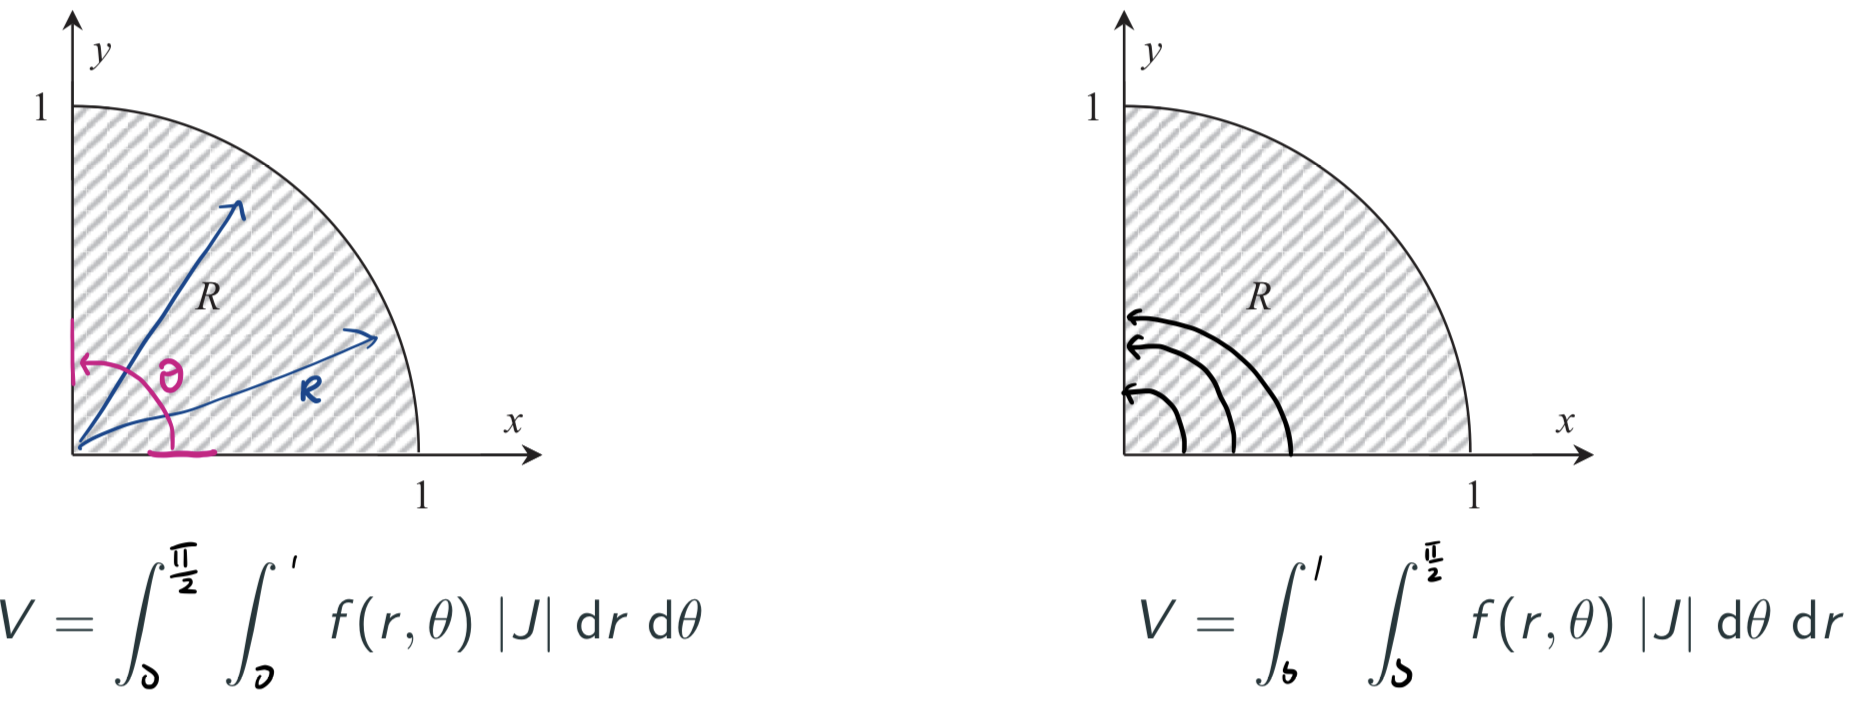
\includegraphics{C:/Users/benmc/iCloudDrive/Uni/obsidian/uni/PNG image.png}\\
where {\(|J|\)} is the absolute value of the \emph{Jacobian} - A
stretching/scaling factor that accounts for the differences between
coordinate systems. It is the determinant of the matrix of first-order
partial derivatives.

\[J = \frac{\partial(x,y)}{\partial(u,v)} = \left| \begin{matrix}
\frac{\partial x}{\partial u} & \frac{\partial x}{\partial v} \\
\frac{\partial y}{\partial u} & \frac{\partial y}{\partial v} \\
\end{matrix} \right| = \frac{\partial x}{\partial u}\frac{\partial y}{\partial v} - \frac{\partial x}{\partial v}\frac{\partial y}{\partial u}\]

Converting to polar: {\(x = r\cos\theta\)} and {\(y = r\sin\theta\)}
Here the Jacobian is {\(J = r\)}

Process:

\begin{enumerate}
\tightlist
\item
  Identify an appropriate coordinate system.
\item
  Find the Jacobian for the proposed coordinate system
\item
  Substitute the new variables into the integral
\item
  Draw the integration region
\item
  Draw the strips in the direction of the inner integral to find the
  inner limits.
\item
  Add up strips across the region R to find the outer limit.
\end{enumerate}

\begin{longtable}[]{@{}ll@{}}
\toprule\noalign{}
Eq & img \\
\midrule\noalign{}
\endhead
{\(\int_{0}^{1}\int_{0}^{\sqrt{1 - y^{2}}}e^{- x^{2}}e^{- y^{2}}\, dx\, dy\)}
{\(\int_{0}^{\frac{\pi}{2}}\int_{0}^{1}e^{- r^{2}}\underset{J}{\underbrace{r}}\, dr\, d\theta\)}
&
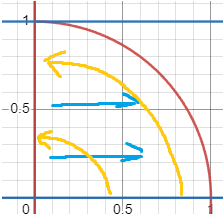
\includegraphics{C:/Users/benmc/iCloudDrive/Uni/obsidian/uni/Pasted image 20230523174627.png} \\
\bottomrule\noalign{}
\end{longtable}
\end{block}
\end{frame}

\begin{frame}{Less obvious Coordinate systems}
\protect\hypertarget{less-obvious-coordinate-systems}{}
Look at the functions boundaries to identify substitutions that give
\hl{constant integral bounds} in the new coordinate system.\\
{\[\int\int_{R}(x^{2} + y^{2})\, dx\, dy\]}Define u, v\\
{\[u = x + y,\, 0 \leq u \leq 2\]}{\[v = x - y,\, 0 \leq v \leq 2\]}Rewrite
in terms of x and y

\[u + v = 2x \rightarrow x = \frac{1}{2}(u + v)\]

\[u - v = 2y \rightarrow y = \frac{1}{2}(u - v)\]

Solve Jacobian

\[J = \left| \begin{matrix}
\frac{\partial x}{\partial u} & \frac{\partial x}{\partial v} \\
\frac{\partial y}{\partial u} & \frac{\partial y}{\partial v} \\
\end{matrix} \right| = \left| \begin{matrix}
\frac{1}{2} & \frac{1}{2} \\
\frac{1}{2} & {- \frac{1}{2}\,} \\
\end{matrix} \right| = - \frac{1}{4} - \frac{1}{4} = - \frac{1}{2}\]

Substitute all variables into original equation\\
{\[\frac{1}{8}\int_{0}^{2}\int_{0}^{2}(u + v)^{2} + (u - v)^{2}\, du\, dv\]}
\end{frame}

\hypertarget{data-analysis}{%
\paragraph{Data Analysis}\label{data-analysis}}

\begin{frame}{Data Analysis}
\begin{block}{Block 1: Statistical Inference}
\protect\hypertarget{block-1-statistical-inference}{}
\begin{itemize}
\item
  Exploratory analysis -- Centre, Spread and Skew
\item
  Core definitions and concepts

  \begin{itemize}
  \tightlist
  \item
    \textbf{P-Value} - The probability that we observe a test statistic
    as least as unusual as the one we have form our sample, given that
    the null hypothesis {\(H_{0}\)} is true.
  \item
    \textbf{Standard Error} - the standard error (of the sample mean) is
    an estimate of the sample-to-sample variability of the sample means
  \item
    \textbf{Confidence Interval} - under repeated sampling, x\% of such
    intervals will contain the true population mean.
  \item
    \textbf{Quantile} - A x\% quantile gives the value of the data, y,
    where x\% of the data (or probability density) is less than or equal
    to y
  \item
    Null and alternative Hypotheses.
    {\(H_{0}:\mu = \text{mean},H_{1}:\mu \neq \text{mean}\)}
  \end{itemize}
\item
  Model formulation, assumptions, and null / alternative hypotheses

  \begin{itemize}
  \tightlist
  \item
    one-sample
  \item
    paired-sample
  \item
    two-sample t-tests.\\
    For each model assumption, identify how we can check the assumption,
    and if they are not satisfied, how we deal with it in our analyses
    (if possible) and what are the consequences for our analyses if they
    are not satisfied?
  \end{itemize}
\item
  Assumptions:\\
  - Independence -\\
  - Normality -\\
  - Equal Variance -\\
  • Understand how Q-Q plots are generated.\\
  • Recognise when we should use the Welch version of the two-sample
  t-test.\\
  • Recall the Central Limit Theorem, and recognise why it is useful for
  our data analyses. What assumption\\
  does it allow us to satisfy?
\end{itemize}

Block 2: Simple Linear Regression\\
This forms the foundation of the DA topics for MM2 and MM3...\\
• Be able to express linear models in terms of an algebraic expression
(y = β0 + β1x) and in terms of R\\
syntax (y ∼ x), and understand how these are related.\\
• Understand what the residual of an observation is, and how this
relates to least squares.\\
• The assumptions of the linear model -- all conveniently expressed in
εi iid\\
∼ N (0, σ2), and how to check\\
for these using appropriate diagnostic plots.\\
• The impact of influential observations in the linear model, and the
rule of thumb used to identify (Cook's\\
D \textgreater{} 0.4) and then check for the point's influence (change
coefficients by 1 se).\\
• Interpreting the p-values from summary() -- recall H0 for these
statistical tests.\\
• Interpreting confidence intervals for regression coefficients.\\
• The R2 statistic: what it means, when is it appropriate to interpret
this, and the rule of thumb that\\
relates R2 to prediction.\\
-- How does R2 relate to the null model?\\
-- what is the null model and how does this relate to the one-sample
t-test?\\
• Carry out a prediction for a given set of x values using regression.\\
-- When should we use a confidence interval? A prediction interval?\\
-- When is it not appropriate to carry out a prediction?\\
Page 1 of 3

Block 3: Multiplicative Models\\
• When is it appropriate to fit a multiplicative model (regression with
a logged response)?\\
What are the tell-tale features in exploratory diagnostic plot(s)?\\
• How should back-transformed confidence intervals be interpreted?\\
-- Effects (e.g. regression coefficients): median in multiplicative /
percentage change terms.\\
-- Predictions: medians\\
Block 4: Categorical Models / One-way ANOVA\\
• How are dummy variables used to model explanatory variables that is
categorical / a factor?\\
-- Given n levels of the factor, how many dummy variables are needed?\\
-- Write down the regression model equation -- both R syntax and
algebraically.\\
• Interpreting summary() output for factors. Why do we need to rotate
factors? How might we tell that\\
this has been done?\\
• Write down the effects model for one-way ANOVA and contrast this with
the regression equation.\\
• Interpret the F -test p-value from anova() (or summary1way() in past
exams). What is the null hy-\\
pothesis? Why is this required when we have 3 or more levels in the
factor?\\
• Understand how total variation is partitioned in the F -test in
anova(), and what this means.\\
• Describe the multiple comparison problem, and how Tukey intervals help
address this problem.\\
• If we have a factor with two levels, then is there a difference in the
results from various approaches for\\
analysis?\\
Block 5: Introduction to Machine Learning -- NEW SINCE 2021!\\
• Describe the differences in how model quality is measured in
statistics and in machine learning.\\
• Explain how an estimate of model quality in ML can be obtained, both
in terms of how errors are\\
measured, and how it is done procedurally.\\
• What is cross-validation? Why do we care about this?\\
• Understand what the following concepts mean, and be able to discuss
this in the context of applications:\\
-- Feature and Target Engineering\\
-- Bias-variance trade-off\\
-- Missing data and possible effects\\
-- Class imbalance\\
-- Data bias\\
-- Historical bias and ethics\\
General\\
• Our general approach to data analysis -- exploratory; fit model; check
assumptions (and transform if\\
justified); do inference.\\
• Writing Executive Summaries.\\
-- In invigilated tests/exams, I will only ask for the Executive
Summary; the content that would\\
go into a Methods and Assumptions Check report will be tested in
specific questions.\\
-- Marks will be deducted for writing reports that you were not asked
for. Do not do brain-dumps.\\
You will NOT be asked questions about:\\
• writing R code.\\
• rote-learning mathematical expressions.\\
• integrating probabilty distribution functions to calculate
probabilites by hand.\\
• calculating quantiles and drawing Q-Q plots by hand.\\
• completing missing entries in an ANOVA table.\\
Page 2 of 3

Please note...\\
• Simple linear regression was introduced into MM2 in 2017.\\
A selection of re-adapted exam questions are available on Canvas.\\
• 2017 S1 Exam Q9's cubic model is not examinable, and there won't be a
question like 2018 S1 Test 2\\
Q2 in style.\\
• The test and exam will follow a similar style to previous semesters
for the most part. There will be\\
short-answer conceptual questions, and you will be writing 1-2 Executive
Summaries.\\
• Shapiro-Wilk test (for normality) and Levene's test (for equal
variance) are no longer examinable.\\
• I suggest using the Practice Problems Book as a starting point for
your revision.\\
• I also suggest using the case studies not discussed in class as extra
practice for writing executive\\
summaries. Remember the introduction does not have to be very long.\\
• Exam solutions are not available for this module. For conceptual
questions, refer to your lectures. For\\
executive summaries, refer to the many examples in your coursebook and
the tutorials. Commentary\\
recordings on some past exams will be available for exam revision. To
avoid disappointment,\\
please do not ask us to provide exam solutions
\end{block}
\end{frame}

\end{document}
